\documentclass[12pt]
{charter}
 

% El títulosde la memoria, se usa en la carátula y se puede usar el cualquier lugar del documento con el comando \ttitle
\titulo{SPCP: Sistema Probabilístico y de ML para Seguimiento y Control de Proyectos} 


\posgrado{Carrera de Especialización en Inteligencia Artificial}

% Tu nombre, se puede usar el cualquier lugar del documento con el comando \authorname
% IMPORTANTE: no omitir titulaciones ni tildación en los nombres, también se recomienda escribir los nombres completos (tal cual los tienen en su documento)
\autor{Lic. Osvaldo Daniel Muñoz}

% El nombre del director y co-director, se puede usar el cualquier lugar del documento con el comando \supname y \cosupname y \pertesupname y \pertecosupname
\director{MBA Ing. Luis Villanueva Canales}
\pertenenciaDirector{Capgemini North Latam} 
\codirector{} % para que aparezca en la portada se debe descomentar la opción codirector en los parámetros de documentclass
\pertenenciaCoDirector{FIUBA}

% Nombre del cliente, quien va a aprobar los resultados del proyecto, se puede usar con el comando \clientename y \empclientename
\cliente{Ing. Fernando Calatayud Cataño}
\empresaCliente{ITSC Digital Value}
 
\fechaINICIO{26 de agosto de 2025}		%Fecha de inicio de la cursada de GdP \fechaInicioName
\fechaFINALPlan{14 de octubre de 2025} 	%Fecha de final de cursada de GdP
\fechaFINALTrabajo{TBD}	%Fecha de defensa pública del trabajo final

\begin{document}
\sloppy
\maketitle
\thispagestyle{empty}
\pagebreak


\thispagestyle{empty}
{\setlength{\parskip}{0pt}
\tableofcontents{}
}
\pagebreak


\section*{Registros de cambios}
\label{sec:registro}

\begin{table}[ht]
\label{tab:registro}
\centering
\begin{tabularx}{\linewidth}{@{}|c|X|c|@{}}
\hline
\rowcolor[HTML]{C0C0C0}
\textbf{Revisión} & \textbf{Detalles de los cambios realizados} & \textbf{Fecha} \\ \hline
0 & Creación del documento & \fechaInicioName \\ \hline
1 & Se completa hasta el punto 5 inclusive & 10 de septiembre de 2025 \\ \hline
%		  Se puede agregar algo más \newline
%		  En distintas líneas \newline
%		  Así                                                    & {día} de {mes} de 202X \\ \hline
%3      & Se completa hasta el punto 12 inclusive                & {día} de {mes} de 202X \\ \hline
%4      & Se completa el plan	                                 & {día} de {mes} de 202X \\ \hline

% Si hay más correcciones pasada la versión 4 también se deben especificar acá


\end{tabularx}
\end{table}

\pagebreak

\section*{Acta de constitución del proyecto}
\label{sec:acta}

\begin{flushright}
CDMX, \fechaInicioName
\end{flushright}

\vspace{2cm}

Por medio de la presente se acuerda con el \authorname\hspace{1px} que su Trabajo Final de la \degreename\hspace{1px} se titulará ``\ttitle'' y consistirá en diseñar y validar un sistema de estimación probabilística para la gestión de proyectos que, a partir de evidencias observadas en el tiempo, entregue pronósticos calibrados y accionables, buscando mejorar con modelos de ML la calibración de las predicciones, indicadores y ratios. El trabajo tendrá un presupuesto preliminar estimado de \textcolor{red}{TBD} horas y un costo estimado de \textcolor{red}{\$ XXX}, con fecha de inicio el \fechaInicioName\hspace{1px} y fecha de presentación pública el \textcolor{red}{\fechaFinalName}.

Se adjunta a esta acta la planificación inicial.

\vfill

% Esta parte se construye sola con la información que hayan cargado en el preámbulo del documento y no debe modificarla
%\begin{table}[ht]
%\centering
%\setlength{\extrarowheight}{2pt}
%\begin{tabular}{@{}ccc@{}}
%\begin{tabular}[c]{@{}c@{}}Dr. Ing. Ariel Lutenberg \\ Director posgrado FIUBA\end{tabular}
%& \hspace{2cm}
%& \begin{tabular}[c]{@{}c@{}}\clientename \\ \empclientename\end{tabular} \\[2.5cm]
%\multicolumn{3}{c}{\begin{tabular}[c]{@{}c@{}}\supname \\ Director del Trabajo Final\end{tabular}} \
%\[2.5cm]
%\end{tabular}
%\end{table}


% Esta parte se construye sola con la información que hayan cargado en el preámbulo del documento y no debe modificarla
\begin{table}[ht]
\centering
\begin{tabular}{ccc}
\begin{tabular}[c]{@{}c@{}}Dr. Ing. Ariel Lutenberg \\ Director posgrado FIUBA\end{tabular} & \hspace{2cm} & \begin{tabular}[c]{@{}c@{}}\clientename \\ \empclientename \end{tabular} \vspace{2.5cm} \\ 
\multicolumn{3}{c}{\begin{tabular}[c]{@{}c@{}} \supname \\ Director del Trabajo Final\end{tabular}} \vspace{2.5cm} \\
\end{tabular}
\end{table}


\section{1. Descripción técnica-conceptual del proyecto a realizar}
\label{sec:descripcion}

\subsection{Introducción}

La compañía \empclientename\hspace{1px} ofrece servicios de (PMO) \eng{Project Management Office} para la planificación, gestión, control y entrega de proyectos de tecnologías de la información bajo los estándares y mejores prácticas dictadas por el PMI (\eng{Project Management Institute}), desarrolladas en su guía PMBOK (\eng{Project Management Body Of Knowledge}).

Los lineamientos del PMI establecen el ciclo de vida de un proyecto en 5 fases, que se representan en la figura 1, y donde delimitamos el alcance de este proyecto a las fases 3 de ejecución, y 4 de monitoreo y control:

% Estilos TikZ
\tikzset{
  fase/.style      = {rectangle, rounded corners, minimum width=3.4cm,
                      minimum height=1.1cm, text centered, draw=black, fill=blue!20},
  resaltada/.style = {fase, fill=orange!35},
  arrow/.style     = {thick, -{Stealth}}
}

\begin{figure}[h]
  \centering

  \begin{tikzpicture}[node distance=2.6cm]

    % Nodos (fases PMI/PMBOK)
    \node (inicio) [fase] {1. Inicio};
    \node (plan)   [fase, right of=inicio, xshift=5.2cm] {2. Planificación};
    \node (exec)   [resaltada, below of=plan, yshift=-2.2cm] {3. Ejecución};
    \node (mon)    [resaltada, left of=exec, xshift=-5.2cm] {4. Monitoreo y Control};
    \node (close)  [fase, below of=mon, yshift=-2.2cm] {5. Cierre};

    % Flechas principales
    \draw [arrow] (inicio) -- (plan);
    \draw [arrow] (plan)   -- (exec);
    \draw [arrow] (exec)   -- (mon);
    \draw [arrow] (mon)    -- (close);

    % Retroalimentación (curva desde Monitoreo a Planificación)
    \draw [arrow, dashed] (mon.north east) .. controls +(2,2) and +(2,-2) .. (plan.south east);

  \end{tikzpicture}

  \caption{Ciclo de vida de un proyecto según PMI/PMBOK. Fases 3 (Ejecución) y 4 (Monitoreo y Control) como alcance del proyecto.}
  \label{fig:ciclo-pmi}
\end{figure}

\subsection{Motivación}

En su recorrido profesional, los \eng{projects managers} han tenido que enfrentar retos y desafíos íntimamente relacionados a la gestión, seguimiento y control de proyectos, en los que la planificación se realiza  principalmente con argumentos y bases de verosimilitud razonable, pero en el despliegue surgen desfases, incumplimientos y subestimaciones, entre otros factores, que derivan en impactos como:

\begin{itemize}
	\item Objetivos estratégicos.
	\item Reprogramación de entregables y sus fechas.
	\item Sobrecostos.
	\item Incumplimiento parcial o total de la relación costo/beneficio establecida.
	\item Credibilidad y confianza en el equipo de trabajo.
	\item Otras iniciativas dependientes en la organización.
\end{itemize}

En este sentido, podemos identificar que los métodos clásicos de la gestión de proyectos tienen limitaciones por el enfoque determinístico, y no proporcionan suficiente información ni predicciones asertivas para tomar decisiones oportunas que mitiguen y/o eviten los impactos en los proyectos descriptos en el párrafo anterior. 

\subsection{El cliente}

\empclientename\hspace{1px} es una empresa mexicana fundada en el año 2013 a la que los clientes le solicitan servicios de consultoría en \eng{project management} (PM). Su \eng{staff} de profesionales generalmente son ingenieros certificados en las metodologías del PMI/PMBOK, y en ocasiones también en tecnologías específicas que les permiten desarrollar su labor principal como PM, así como el complemento de conocimientos específicos como telecomunicaciones o ingeniería civil para proyectos de construcción.

La misión y visión de la empresa está expresada en estos términos en la figura 2:

\begin{figure}[htpb]
\captionsetup{justification=centering,singlelinecheck=false}
\centering 

\includegraphics[width=\textwidth]{./Figuras/ITSC_Mision_Vision.pdf}
\caption{Misión y visión de ITSC Digital Value.}
\label{fig:ITSC_Mision_Vision}
\end{figure}

\subsection{Situación actual (\eng{as-is})}

El macro proceso clásico compuesto de 5 fases para la gestión de proyectos, según los lineamientos del PMI/PMBOK, es el que adoptan y despliegan los profesionales asignados a los contratos con los clientes, como se ve en la figura 3:

% =========================
% Figura 1: Macro-proceso
% =========================
\begin{figure}[h]
\centering
\begin{adjustbox}{max width=\linewidth} % asegura que no desborde
\begin{tikzpicture}[node distance=1.8cm and 0.8cm]
  \node (f1) [fase]{1. Inicio};
  \node (f2) [fase, right=of f1]{2. Planificaci\'on};
  \node (f3) [fase, right=of f2]{3. Ejecuci\'on};
  \node (f4) [fase, right=of f3, text width=3.2cm, align=center]{4. Monitoreo y Control};
  \node (f5) [fase, right=of f4]{5. Cierre};
  \draw[arr] (f1) -- (f2);
  \draw[arr] (f2) -- (f3);
  \draw[arr] (f3) -- (f4);
  \draw[arr] (f4) -- (f5);
\end{tikzpicture}
\end{adjustbox}
\caption{Macro-proceso del ciclo de vida de un proyecto (PMI/PMBOK).}
\label{fig:macro-pmi}
\end{figure}

\FloatBarrier

Las entradas y salidas que requieren y generan cada una de las cinco fases se describen en las figuras 4 a 8 como sigue: 

% --- Fase 1: Inicio ---
\begin{figure}[h]
\centering
\pmiFaseH{1. Inicio}
        {Business case\\Contratos / acuerdos\\EEF, OPA}
        {Acta de constituci\'on (Project Charter)\\Registro de interesados}
\caption{Fase 1: Inicio — Entradas y salidas principales.}
\label{fig:fase1}
\end{figure}

% --- Fase 2: Planificación ---
\begin{figure}[h]
\centering
\pmiFaseH[fill=blue!22]{2. Planificaci\'on}
        {Acta de constituci\'on\\Registro de interesados\\Requisitos iniciales\\EEF, OPA}
        {Plan para la direcci\'on del proyecto\\L\'ineas base (alcance/tiempo/costo)\\EDT/WBS\\Registro de riesgos\\Planes subsidiarios (calidad, recursos,\\comunicaciones, adquisiciones, interesados, etc.)}
\caption{Fase 2: Planificaci\'on — Entradas y salidas principales.}
\label{fig:fase2}
\end{figure}

% --- Fase 3: Ejecución ---
\begin{figure}[h]
\centering
\pmiFaseH[fill=orange!25]{3. Ejecuci\'on}
        {Plan para la direcci\'on del proyecto\\L\'ineas base\\Documentos del proyecto}
        {Entregables\\Datos/Informaci\'on de desempe\~no (WPD/WPI)\\Solicitudes de cambio\\Actualizaciones al plan y documentos}
\caption{Fase 3: Ejecuci\'on — Entradas y salidas principales.}
\label{fig:fase3}
\end{figure}

% --- Fase 4: Monitoreo y Control ---
\begin{figure}[h]
\centering
\pmiFaseH[fill=orange!25]{4. Monitoreo y Control}
        {Plan de gesti\'on\\Datos/Informaci\'on de desempe\~no}
        {Informes de desempe\~no (Reports)\\Cambios aprobados / rechazados\\Acciones correctivas / preventivas\\Actualizaciones (plan, documentos, OPA)}
\caption{Fase 4: Monitoreo y Control — Entradas y salidas principales.}
\label{fig:fase4}
\end{figure}

% --- Fase 5: Cierre ---
\begin{figure}[h]
\centering
\pmiFaseH[fill=blue!22]{5. Cierre}
        {Entregables aceptados\\Documentaci\'on del proyecto}
        {Producto/servicio final transferido\\Cierre de proyecto/fase documentado\\Lecciones aprendidas (OPA)\\Liberaci\'on de recursos}
\caption{Fase 5: Cierre — Entradas y salidas principales.}
\label{fig:fase5}
\end{figure}

\FloatBarrier

De acuerdo a la experiencia del cliente, los proyectos se gestionan en las fases 3 (ejecución) y 4 (monitoreo y control), con un grado de incertidumbre variable, dependiendo de:

\begin{itemize}
	\item La complejidad.
	\item Experiencia de los recursos asignados.
	\item Claridad y fluidez en la comunicación.
	\item Grado de compromiso hacia la producción de los entregables.
	\item Disponibilidad oportuna de los recursos financieros y materiales presupuestados.
	\item Eficiencia del modelo de gobierno.
	\item Habilidades y conocimientos de la oficina de gerencia del proyecto (PMO).
\end{itemize}

Debido a los grados de incertidumbre que existen en las fases 3 y 4 de la gestión de proyectos, el cliente requiere contar con un modelo que le proporcione, a partir de los datos que genera el modelo clásico, información complementaria y confiable mediante indicadores y ratios para tomar decisiones oportunas. 
Y de esta menera poder anticipar, mitigar y, en lo posible, evitar los desvíos e impactos en los resultados esperados del proyecto en cuanto a alcance, tiempo, costo y calidad propuestos al inicio en el \eng{statement of work} (SOW).

\subsection{Preguntas centrales}

Dado el historial de un proyecto y sus artefactos:

\begin{itemize}
	\item ¿Cuál es la probabilidad de exceder el baseline vigente en cada dimensión (tiempo, alcance, costo)?
	\item ¿Cómo evolucionan los indicadores de riesgos e incidentes para anticipar desvíos?
    \item Con modelos de \eng{machine learning} (ML) (\eng{boosting} cuantílico; TCN/LSTM), ¿mejoran el error y la calibración de los pronósticos de $\tfrac{\Delta_d}{EAC}$ y $P(\text{atraso/sobrecosto})$ frente a EVM/PERT/ARIMA?
\end{itemize}

\subsection{Estado del arte}

Aunque los métodos estadísticos clásicos constituyen una base sólida, resultan limitados para capturar no linealidades y efectos de interacción entre variables (p. ej., SPI/CPI, cambios de alcance, riesgos, incidentes). En este contexto, los enfoques de ML tabular y secuencial permiten explotar dichas interacciones y patrones temporales, ofreciendo bandas de predicción y probabilidades mejor calibradas. Asimismo, se priorizará la interpretabilidad (SHAP, PDP) y se establecerán comparaciones rigurosas frente a los baselines estadísticos, en línea con el enfoque requerido.

La figura 9 es un esquema de bloques de la solución propuesta:

% State of the art
\begin{figure}[h]
\centering
\begin{adjustbox}{max width=\textwidth, center}
\begin{tikzpicture}[
  font=\small,
  box/.style     = {rectangle, rounded corners=12pt, draw=black!60, thick, fill=white,
                    text width=9cm, align=left, minimum height=1.2cm, inner sep=6pt},
  highlight/.style = {box, draw=blue!60,   fill=blue!10},
  risk/.style      = {box, draw=orange!70, fill=orange!10},
  outp/.style      = {box, draw=green!60!black, fill=green!10},
  arr/.style       = {-{Stealth}, thick},
  darr/.style      = {-{Stealth}, thick, dashed}
]

% ---------- COLUMNA CENTRAL ----------
\node (H1) [box] at (0,0) {\textbf{Fuente de Datos}\\ CSV / DB / PMIS / APIs};
\node (A1) [box,      below=12mm of H1]
      {\textbf{1) Ingesta de Datos}\\ PV, EV, AC, BAC, Fechas\\ CPI, SPI, CV, SV, rolling};
\node (B1) [highlight, below=12mm of A1]
      {\textbf{2) Capa Probabilística (Bayes/MC)}\\ EAC como distribución (P50–P80–P90)\\ S-curves, $P(\text{Finish}>\text{Baseline})$};
\node (C1) [box,      below=12mm of B1]
      {\textbf{3) Capa ML}\\ XGBoost / RF / LSTM\\ Pred. $\Delta$Costo, $\Delta$Tiempo\\ Explicabilidad (SHAP)};
\node (D1) [risk,     below=12mm of C1]
      {\textbf{4) Gobernanza (PMBOK M\&C)}\\ Control Costs (TCPI prob.)\\ Control Schedule (P50/P80)\\ Monitor Risks\\ Change Control};
\node (E1) [outp,     below=12mm of D1]
      {\textbf{5) Visualización / Reporting}\\ Dashboards, histogramas, S-curves\\ Tablas P50/P80/P90};
\node (F1) [box,      below=12mm of E1]
      {\textbf{6) Validación / Benchmark}\\ EVM clásico vs Bayes vs ML\\ MAE, RMSE, Calibración};
\node (G1) [box,      below=12mm of F1]
      {\textbf{Repositorio Reproducible}\\ Git / DVC / Experimentos};

% Flechas principales
\draw[arr] (H1) -- (A1);
\draw[arr] (A1) -- (B1);
\draw[arr] (B1) -- (C1);
\draw[arr] (C1) -- (D1);
\draw[arr] (D1) -- (E1);
\draw[arr] (E1) -- (F1);
\draw[arr] (F1) -- (G1);

% ---------- COORDENADAS LATERALES (guías simétricas) ----------
\coordinate (Ledge) at ($(A1.west)+(-2.8cm,0)$); % misma distancia a ambos lados
\coordinate (Redge) at ($(A1.east)+( 2.8cm,0)$);

% ---------- BACK-ITERATION IZQUIERDA: 5 -> 1 (con etiqueta centrada en el tramo vertical) ----------
\coordinate (L1)    at ($ (E1.west) + (-2mm,0) $);
\coordinate (L2)    at ($ (A1.west) + (-2mm,0) $);
\coordinate (LLtop) at (Ledge |- L1);
\coordinate (LLbot) at (Ledge |- L2);

\draw[darr] (E1.west) -- (L1) -- (LLtop) -- (LLbot) -- (A1.west);
\node[
  fill=white, draw=white, rounded corners=2pt,
  inner sep=2pt, text width=3.0cm, align=center
] at ($ (LLtop)!0.5!(LLbot) $) {\footnotesize Retroalimentación\\ Ajustes de baseline};

% ---------- BACK-ITERATION DERECHA: 5 -> 4 (simétrico al izquierdo) ----------
\coordinate (R1)    at ($ (E1.east) + ( 2mm,0) $);
\coordinate (R2)    at ($ (D1.east) + ( 2mm,0) $);
\coordinate (RRtop) at (Redge |- R1);
\coordinate (RRbot) at (Redge |- R2);

\draw[darr] (E1.east) -- (R1) -- (RRtop) -- (RRbot) -- (D1.east);
\node[
  fill=white, draw=white, rounded corners=2pt,
  inner sep=2pt, text width=3.0cm, align=center
] at ($ (RRtop)!0.5!(RRbot) $) {\footnotesize Iteración local\\ Comité de control};

\end{tikzpicture}
\end{adjustbox}
\caption{\eng{To-be} - esquema vertical en bloques de la solución propuesta.}
\end{figure}

\FloatBarrier

\subsection{Glosario de siglas}

\begin{table}[h]
\centering
\caption{Siglas utilizadas en esta documento y su significado}
\begin{tabularx}{\textwidth}{lY}
\toprule
\textbf{Sigla} & \textbf{Concepto / significado} \\
\midrule
PMI & \textit{Project Management Institute}. \\
PMBOK & \textit{Project Management Body of Knowledge}. \\
WBS/EDT & \textit{Work Breakdown Structure} / Estructura de Desglose del Trabajo. \\
AoN & \textit{Activity on Node} (Diagrama de actividades con nodos). \\
PV & \textit{Planned Value} (Valor planificado) — valor del trabajo planificado a la fecha \;[\$]. \\
EV & \textit{Earned Value} (Valor ganado) — valor del trabajo realmente completado \;[\$]. \\
AC & \textit{Actual Cost} (Costo real) — costo incurrido a la fecha \;[\$]. \\
BAC & \textit{Budget at Completion} (Presupuesto al completar) \;[\$]. \\
CPI & \textit{Cost Performance Index} — $CPI = EV/AC$ (>\,1 = eficiente). \\
SPI & \textit{Schedule Performance Index} — $SPI = EV/PV$ (>\,1 = adelantado). \\
CV & \textit{Cost Variance} — $CV = EV - AC$ \;[\$]. \\
SV & \textit{Schedule Variance} — $SV = EV - PV$ \;[\$]. \\
EAC & \textit{Estimate at Completion} (Estimación al completar). \\
ETC & \textit{Estimate to Complete} — $ETC = EAC - AC$ \;[\$]. \\
VAC & \textit{Variance at Completion} — $VAC = BAC - EAC$ \;[\$]. \\
TCPI & \textit{To-Complete Performance Index} (Índice de desempeño requerido). \\
PERT & Duraciones $a,m,b$ (optimista, más probable, pesimista) para Beta–PERT. \\
P50/P80/P90 & Percentiles de costo/fecha (medidas probabilísticas). \\
RPN & \textit{Risk Priority Number} — $RPN = S \times O$ (Severidad $\times$ Ocurrencia). \\
ML & \textit{Machine Learning}. \\
\bottomrule
\end{tabularx}
\end{table}

\FloatBarrier

\subsection*{Fórmulas e interpretación}

\paragraph{Indicadores EVM \textit{Earn Value Management}}
\[
\begin{aligned}
CPI &= \frac{EV}{AC} \quad & (>1\ \text{favorable, eficiencia de costo})\\
SPI &= \frac{EV}{PV} \quad & (>1\ \text{adelantado en cronograma})\\[2pt]
CV  &= EV - AC              & (\text{\$ positivo = ahorro, negativo = sobrecosto})\\
SV  &= EV - PV              & (\text{\$ positivo = adelantado, negativo = atraso})
\end{aligned}
\]

\paragraph{Pronósticos de costo}
\begin{table}[h]
\centering
\begin{tabularx}{\textwidth}{>{$}l<{$} Y}
\toprule
\displaystyle EAC_1 = \frac{BAC}{CPI} & Asume que el desempeño actual de costos continúa \\
\displaystyle EAC_2 = AC + (BAC - EV) & Asume ejecución futura al costo presupuestado \\
\displaystyle EAC_{CPI\cdot SPI} = AC + \frac{BAC - EV}{CPI \cdot SPI} & Si el atraso de cronograma impacta costos \\
\displaystyle ETC = EAC - AC;\ \ VAC = BAC - EAC & Definiciones derivadas \\
\bottomrule
\end{tabularx}
\end{table}


\paragraph{Índice de desempeño requerido (TCPI)}
\[
\begin{aligned}
TCPI_{BAC} &= \frac{BAC - EV}{BAC - AC}
&& \text{(para cumplir con el BAC original)}\\
TCPI_{EAC} &= \frac{EAC - EV}{EAC - AC}
&& \text{(para cumplir con un nuevo objetivo EAC)}
\end{aligned}
\]
\textit{Lectura:} $TCPI>1$ implica \textbf{presión de costo}, será necesario mejorar la eficiencia para alcanzar la meta (BAC/EAC); $TCPI<1$ implica \textbf{margen de costo}, es posible cumplir, aun con una eficiencia menor a la actual.

\paragraph{PERT (duraciones) y Monte Carlo}
Para una actividad con estimaciones $(a,m,b)$:
\[
\mu = \frac{a + 4m + b}{6}, \qquad \sigma^2 = \frac{(b - a)^2}{36}.
\]
Sumando actividades (suposición simple de independencia): $\mu_{\text{proy}} = \sum \mu_i$, $\ \sigma_{\text{proy}} = \sqrt{\sum \sigma_i^2}$. En la práctica, usar \emph{Monte Carlo} para capturar dependencias y así obtener percentiles de fecha/costo ($P50$, $P80$, $P90$).

\paragraph{Percentiles y S-curves}
Reportando costo/fecha como distribución: por ejemplo, “Costo P50 = \$X, P80 = \$Y; $P(\text{EAC} > BAC)=z\%$”. Esto reemplaza el número único por rangos accionables.

\FloatBarrier


\section{2. Identificación y análisis de los interesados}
\label{sec:interesados}

\begin{table}[ht]
\setlength{\extrarowheight}{2pt}
\begin{tabularx}{\linewidth}{@{}|l|T|T|l|@{}}
\hline
\rowcolor[HTML]{C0C0C0} 
Rol           & Nombre y Apellido & Organización & Puesto \\ \hline
Cliente       & \nohyphens{\clientename} & \nohyphens{\empclientename} & Director de Operaciones \\ \hline
Responsable   & \nohyphens{\authorname} & FIUBA                  & Alumno \\ \hline
Orientador    & \nohyphens{\supname} & \nohyphens{\pertesupname} & Director del Trabajo Final \\ \hline
Equipo        & \makecell[l]{TBD 1\\TBD 2} & \makecell[c]{\textemdash} & \makecell[c]{\textemdash} \\ \hline
Opositores    & \eng{Team leaders} & Cliente y \eng{contractors} & \makecell[c]{\textemdash} \\ \hline
Usuario final & \eng{Project Managers} & \empclientename & \makecell[c]{\textemdash} \\ \hline
\end{tabularx}
\end{table}

\FloatBarrier

\begin{itemize}
	\item Orientador: el MBA Ing. Luis Villanueva Canales es un reconocido profesional en ciencias de la computación y electrónica y colaborará en refinar los requerimientos, así como dar las guías desde su experiencia para lograr los propósitos del proyecto.
	\item Cliente: el Ing. Fernando Calatayud Cataneo es exigente y detallista con vasta experiencia en entrega de servicios de consultoría. Conoce en profundidad los retos y desafíos de las disciplinas, con lo cual será riguroso en la definición de los requerimientos y en la calidad del producto final.
	\item Equipo: el equipo de trabajo se definirá a partir del dimensionamiento de las áreas de conocimiento que requiera el proyecto para su construcción. Es muy importante tener las definiciones para poder seleccionarlo.
\end{itemize}


\section{3. Propósito del proyecto}
\label{sec:proposito}

Diseñar y validar un sistema de estimación probabilística que, a partir de evidencias observadas en el tiempo, entregue pronósticos calibrados y accionables, buscando mejorar con modelos de ML la calibración de las predicciones, indicadores y ratios.

\section{4. Alcance del proyecto}
\label{sec:alcance}

El proyecto incluye:
\begin{itemize}
	\item Formalizar las variables y artefactos (\eng{work breakdown structure} (WBS), cronograma, costo, registros de riesgo/incidentes, cambios).
	\item Definir un modelo de probabilidad de desvío por dimensión $(\text{tiempo} / \text{alcance} / \text{costo})$ y su relación con riesgos/incidentes.
	\item Entrenar y validar modelos $(\text{Bayes} / \text{Monte Carlo} / \text{series de tiempo})$ con \eng{backtesting}.
	\item Evaluar calibración y utilidad (curvas S con bandas, alertas tempranas, what-if).
	\item Entregar un tablero/notebooks reproducibles y una guía de uso para PMs. 
\end{itemize}

El proyecto no incluye:
\begin{itemize}
	\item Proyectos sin \eng{baseline}.
	\item Datos no estructurados, o si no es posible normalizarlos.
	\item Estimación de recursos humanos a nivel individual (si hubiera faltante de datos). 
\end{itemize}

\section{5. Supuestos del proyecto}
\label{sec:supuestos}

Para el desarrollo del presente proyecto se establecen las siguientes hipótesis:

\begin{itemize}
	\item La inclusión de variables de riesgo e incidentes mejora la predicción de desvíos en plazo y costo.
	\item Un modelo jerárquico bayesiano por paquete de trabajo (WBS) produce estimaciones mejor calibradas que una línea de base determinista + tendencia.
	\item Dado que el \eng{boosting} cuantílico aprende relaciones no lineales e interacciones (SPI, CPI, $\Delta_{\text{scope}}$, riesgos, incidentes) y genera bandas de predicción directamente, luego entonces, mejora la cobertura $(q_{10}/q_{50}/q_{90})$ y CRPS (\eng{Continuous Ranked Probability Score}).
	\item $\text{TCN} / \text{LSTM}$ ($\text{\eng{Temporal Convolutional Network}} / \text{\eng{Long Short-Term Memory}}$) reduce el \eng{Mean Absolute Error} (MAE) cuando existen dependencias temporales fuertes.
\end{itemize}

% (analizar y revisar donde va este criterio) Criterio de decisión: se privilegiarán modelos con mejor calibración (\eng{Expected Calibration Error} (ECE) / cobertura) y de utilidad para el PM (alertas útiles), aun si los métodos clásicos fueran competitivos.

\section{6. Requerimientos}
\label{sec:requerimientos}

\subsection{Funcionales (FR)}
\begin{description}
  \item[\textbf{FR-01 Ingesta al modelo unificado (DER vigente)}] El sistema debe aceptar datos por CSV/APIs y normalizarlos al modelo unificado del SPCP, conforme al DER vigente (todas las entidades definidas), aplicando reglas de tipos, obligatorios y PK/FK del diccionario.

  \item[\textbf{FR-02 Validación de dataset}] Validar columnas, tipos, PK/FK e impedir acumulados decrecientes (PV/EV/AC).

  \item[\textbf{FR-03 Cálculo EVM}] Calcular CPI, SPI, CV, SV, EAC (variantes) y TCPI.

  \item[\textbf{FR-04 Monte Carlo (cronograma)}] Simular con PERT (a,m,b) $\geq$ 10{,}000 corridas; entregar finish P50/P80/P90 y $P(\text{Finish}>\text{Baseline})$.

  \item[\textbf{FR-05 Bayes (desempeño)}] Actualizar una red bayesiana por corte con observables (CPI, SPI, exposición de riesgo, cambios 7d, retrabajo, demoras proveedor) y estimar $P(\text{EAC}>\text{BAC})$ y \textit{drivers}.

  \item[\textbf{FR-06 ML baseline}] Entrenar un modelo ML (p.ej., XGBoost) para EAC a t+4 semanas y probabilidad de sobrecosto $>10\%$, con importancia/SHAP.

  \item[\textbf{FR-07 Fusión de señales y fiabilidad}] Combinar \textbf{EVM + Bayes + ML} mediante \textit{ensamble} (promedio ponderado o stacking) para producir: (i) \textbf{EAC final} y (ii) \textbf{probabilidad de sobrecosto}. 
  %Aplicar un \textbf{mapeo monotónico (isotónico)} que alinee las probabilidades con las frecuencias observadas en validación, cumpliendo: MAE(EAC) del ensamble $\le$ EVM $-10\%$, cobertura P50 = 45--55\%, P80 = 75--85\%, y Brier $\le 0.18$.

  \item[\textbf{FR-08 Visualización ejecutiva}] El sistema debe presentar un \textbf{panel de indicadores ejecutivos} (KPIs de cabecera: P50/P80/P90 de EAC, $P(\text{EAC}>\text{BAC})$, TCPI), además de \textbf{curvas S}, \textbf{histograma de simulaciones} y una \textbf{tabla ejecutiva} con descarga CSV/PDF.

  \item[\textbf{FR-09 Escenarios}] Permitir \textit{“what-if”} (cambios/riesgos) y recalcular percentiles y $P(\text{EAC}>\text{BAC})$.

  \item[\textbf{FR-10 Cortes y trazabilidad}] Emitir \textbf{cortes semanales} del dataset con \textbf{manifiesto y huella (hash)}, y guardar la \textbf{trazabilidad de cálculos} por corte para asegurar \textbf{reproducibilidad}.

  \item[\textbf{FR-11 Descarga y API}] Permitir la descarga de resultados (CSV/PDF/PNG) y su consulta por API HTTP sencilla.

\end{description}

\subsection{Documentación (DOC)}
\begin{description}
  \item[\textbf{DOC-01 DER y diccionario}] Entregar diagrama de entidad-relación (DER) y diccionario de datos (definiciones, dominios, \textit{Primary Key / Foreign Key} (PK/FK)).

  \item[\textbf{DOC-02 Mapeo de fuentes}] Matriz Origen$\rightarrow$modelo unificado por campo (PMIS/ERP/Jira/HR).

  \item[\textbf{DOC-03 Manual de usuario}] Flujo de carga, validación, ejecución, dashboards y exportaciones con capturas.

  \item[\textbf{DOC-04 Manual de operación}] Jobs, \textit{seeds}, variables, backups, rotación de contraseñas, monitoreo.

  \item[\textbf{DOC-05 DOC-05 — Ficha del modelo y de la red bayesiana}] Datos, métricas, deriva de datos, límites de uso y política de re-entrenamiento; incluir en la ficha de la BN los nodos, observables y supuestos.

  \item[\textbf{DOC-06 Plan de pruebas}] Casos de prueba para todos los requerimientos aplicables (funcionales, interfaz de usuario, integración, no funcionales, etc.), con criterios de aceptación y trazabilidad.

\end{description}

% Seguir aquí

\subsection{Testing (TEST)}
\begin{description}
  \item[\textbf{TEST-01 Pruebas unitarias de ETL}] Cobertura $\geq$ 80\% en los módulos de lectura y normalización de datos (parsers/normalizadores).

  \item[\textbf{TEST-02 Contrato de datos}] Validación del esquema durante la integración continua (CI); el proceso de build debe fallar ante cambios incompatibles.

  \item[\textbf{TEST-03 Validación de la red bayesiana (BN)}] Pruebas de posterior predictivo y análisis de sensibilidad de nodos para verificar la robustez de la BN.

  \item[\textbf{TEST-04 Modelo Monte Carlo}] Ejecuciones reproducibles (uso de semilla y validación de tolerancias en percentiles).

  \item[\textbf{TEST-05 Validación de modelos de ML}] Validación cruzada \textit{k-fold} con reporte de MAE/RMSE y verificación de curva de calibración aceptable.

  \item[\textbf{TEST-06 Backtesting}] Validación \textit{rolling-origin} vs. cortes históricos para EAC/fechas (MAE/RMSE y calibración).

  \item[\textbf{TEST-07 Integración con APIs}] En caso que aplique, pruebas con simulación controlada para Jira/PMIS/ERP, incluyendo casos de borde (valores nulos y duplicados).

  \item[\textbf{TEST-08 Desempeño del panel}] El dashboard inicial debe cargar en $\leq$ 5 segundos (p95) como meta ideal, y $\leq$ 10 segundos (p95) como meta mínima aceptable, para 12 meses de datos y 5,000 actividades.

  \item[\textbf{TEST-09 Seguridad}] Escaneo de dependencias y contraseñas, con verificación de controles básicos de acceso (RBAC)

  \item[\textbf{TEST-10 Pruebas de aceptación de usuario (UAT)}] Ejecución de 10 escenarios de negocio validados y firmados por el cliente.

\end{description}

\subsection{Interfaz de usuario (UI)}
\begin{description}
  \item[\textbf{UI-01 Diseño web adaptable}] Visualización correcta en pantallas desde 1366$\times$768 en adelante; versión móvil de solo lectura.

  \item[\textbf{UI-02 Indicadores claros (KPI)}] Tarjetas con EAC P50/P80/P90, $P(\text{EAC}>\text{BAC})$, TCPI con leyenda.

  \item[\textbf{UI-03 Gráficos principales}] S-curves, histograma de simulaciones, tendencias CPI/SPI y \textit{waterfall} de EAC.

  \item[\textbf{UI-04 Navegación y trazabilidad}] Flujo de exploración: Entregable $\rightarrow$ Actividades $\rightarrow$ Riesgos/Cambios vinculados.

  \item[\textbf{UI-05 Explicabilidad combinada}] Panel de \textbf{SHAP/feature importance} (ML) y sensibilidad bayesiana (efecto de observables en posteriors), acompañado de texto breve.

   \item[\textbf{UI-06 Exportación}] Exportar vistas clave en CSV, PDF y PNG con un solo clic.

\end{description}

\subsection{Datos (DATA)}
\begin{description}
  \item[\textbf{DATA-01 Modelo unificado (DER vigente)}] Usar únicamente las columnas definidas en el esquema oficial; no se permiten campos extra ad-hoc.

  \item[\textbf{DATA-02 Formato de fechas}] Todas las fechas en formato YYYY-MM-DD y status\_date semanal consistente.

  \item[\textbf{DATA-03 Identificadores (IDs)}] Únicos, estables, sin espacios; no reciclar IDs.

  \item[\textbf{DATA-04 Calidad de datoa}] Valores faltantes deben estar explícitos (no NaN); acumulados no pueden decrecer; moneda consistente dentro de cada proyecto.

  \item[\textbf{DATA-05 Temporalidad}] Separar \textit{train/val/test} por tiempo (sin datos futuros); usar solo datos hasta cada fecha de corte.

\end{description}

\subsection{De despliegue/DevOps (DEV)}
\begin{description}
  \item[\textbf{DEV-01 Empaquetado}] Implementación en \textit{Docker}, usando variables de entorno para rutas y credenciales.

  \item[\textbf{DEV-02 Datos de ejemplo (seeds)}] Dataset demo reproducible para pruebas y aceptación de usuario (UAT).
  
  \item[\textbf{DEV-03 Jobs automáticos}] Orquestación del corte semanal y generación de reportes/exportables.
  
  \item[\textbf{DEV-04 Copias de respaldo (backups)}] Retención de snapshots y outputs durante al menos 6 meses, con verificación periódica de restauración.
  
  \item[\textbf{DEV-05 Operaciones de ML (MLOps)}] Registro de modelos, versionado de artefactos (modelo, features, semillas) y política de reentrenamiento.

\end{description}


\section{7. Historias de usuarios (\textit{Product backlog})}
\label{sec:backlog}

La estimación de cada historia se basa en \textbf{complejidad}, \textbf{dificultad} e \textbf{incertidumbre}.
Si la suma excede el máximo usual (20), se revisan las ponderaciones, especialmente la incertidumbre, ajustándolas a la realidad del SPCP donde los datos y modelos ya están definidos.
De esta forma se evita inflar artificialmente las estimaciones y se mantiene la coherencia con la escala de Fibonacci modificada.

\subsection*{Backlog inicial:}

\begin{enumerate}
  \item Como jefe de PMs (cliente interno) quiero comparar el desempeño de todos mis proyectos en un panel consolidado para identificar rápidamente cuáles necesitan intervención.\\
  \textit{Story points: 20 (complejidad 6, dificultad 6, incertidumbre 5)}

  \item Como analista de riesgos quiero ejecutar escenarios \textit{what-if} modificando riesgos o duraciones críticas para ver cómo cambia la probabilidad de sobrecosto.\\
  \textit{Story points: 13 (complejidad 5, dificultad 4, incertidumbre 4)}

  \item Como usuario ejecutivo quiero descargar en un clic un reporte en PDF con la tabla de indicadores clave para llevarlo al comité de control.\\
  \textit{Story points: 8 (complejidad 3, dificultad 2, incertidumbre 3)}

  \item Como administrador del sistema quiero tener cortes semanales versionados con 
  \texttt{manifest + hash} para asegurar trazabilidad y reproducibilidad de resultados.\\
  \textit{Story points: 8 (complejidad 3, dificultad 3, incertidumbre 2)}

  \item Como PM quiero ver un panel con P50/P80/P90 de EAC y \texttt{P(EAC > BAC)} 
  para monitorear rápidamente la proyección de costos de mi proyecto.\\
  \textit{Story points: 5 (complejidad 2, dificultad 2, incertidumbre 1)}

  \item Como usuario externo al sistema quiero consultar un servicio sencillo que me entregue percentiles y alertas para integrar los resultados del SPCP en otras aplicaciones.\\
  \textit{Story points: 5 (complejidad 2, dificultad 2, incertidumbre 1)}
\end{enumerate}

\section{8. Entregables principales del proyecto}
\label{sec:entregables}

\begin{consigna}{red}
Los entregables del proyecto son (ejemplo):

\begin{itemize}
	\item Manual de usuario.
	\item Diagrama de circuitos esquemáticos.
	\item Código fuente del firmware.
	\item Diagrama de instalación.
	\item Memoria del trabajo final.
	\item etc...
\end{itemize}
\end{consigna}

\section{9. Desglose del trabajo en tareas}
\label{sec:wbs}

\begin{consigna}{red}
El WBS debe tener relación directa o indirecta con los requerimientos.  Son todas las actividades que se harán en el proyecto para dar cumplimiento a los requerimientos. Se recomienda mostrar el WBS mediante una lista indexada:

\begin{enumerate}
\item Grupo de tareas 1 (suma h)
	\begin{enumerate}
	\item Tarea 1 (tantas h)
	\item Tarea 2 (tantas h)
	\item Tarea 3 (tantas h)
	\end{enumerate}
\item Grupo de tareas 2 (suma h)
	\begin{enumerate}
	\item Tarea 1 (tantas h)
	\item Tarea 2 (tantas h)
	\item Tarea 3 (tantas h)
	\end{enumerate}
\item Grupo de tareas 3 (suma h)
	\begin{enumerate}
	\item Tarea 1 (tantas h)
	\item Tarea 2 (tantas h)
	\item Tarea 3 (tantas h)
	\item Tarea 4 (tantas h)
	\item Tarea 5 (tantas h)
	\end{enumerate}
\end{enumerate}

Cantidad total de horas: tantas.

\textbf{¡Importante!:} la unidad de horas es h y va separada por espacio del número. Es incorrecto escribir ``23hs".

\textbf{Se recomienda que no haya ninguna tarea que lleve más de 40 h.} De ser así se recomienda dividirla en tareas de menor duración.

\end{consigna}

\section{10. Diagrama de Activity On Node}
\label{sec:AoN}

\begin{consigna}{red}
Armar el AoN a partir del WBS definido en la etapa anterior.

Una herramienta simple para desarrollar los diagramas es el Draw.io (\url{https://app.diagrams.net/}).
\href{https://app.diagrams.net}{Draw.io}


\begin{figure}[htpb]
\centering 
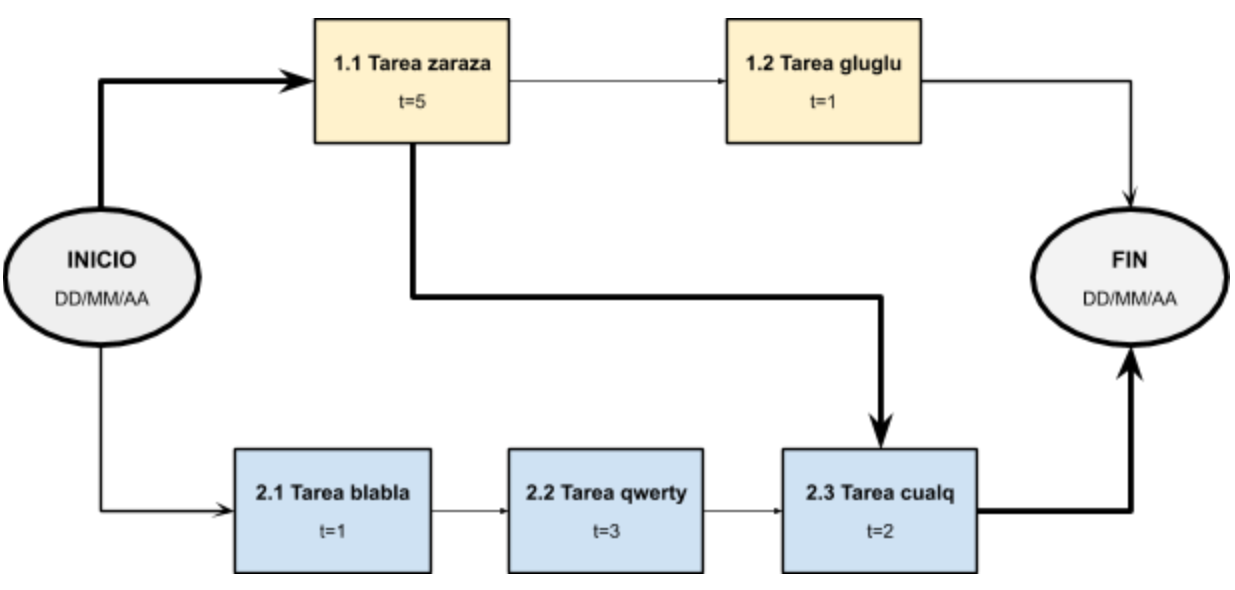
\includegraphics[width=.8\textwidth]{./Figuras/AoN.png}
\caption{Diagrama de \textit{Activity on Node}.}
\label{fig:AoN}
\end{figure}

Indicar claramente en qué unidades están expresados los tiempos.
De ser necesario indicar los caminos semi críticos y analizar sus tiempos mediante un cuadro.
Es recomendable usar colores y un cuadro indicativo describiendo qué representa cada color.

\end{consigna}

\section{11. Diagrama de Gantt}
\label{sec:gantt}

\begin{consigna}{red}
Existen muchos programas y recursos \textit{online} para hacer diagramas de Gantt, entre los cuales destacamos:

\begin{itemize}
\item Planner
\item GanttProject
\item Trello + \textit{plugins}. En el siguiente link hay un tutorial oficial: \\ \url{https://blog.trello.com/es/diagrama-de-gantt-de-un-proyecto}
\item Creately, herramienta online colaborativa. \\\url{https://creately.com/diagram/example/ieb3p3ml/LaTeX}
\item Se puede hacer en latex con el paquete \textit{pgfgantt}\\ \url{http://ctan.dcc.uchile.cl/graphics/pgf/contrib/pgfgantt/pgfgantt.pdf}
\end{itemize}

Pegar acá una captura de pantalla del diagrama de Gantt, cuidando que la letra sea suficientemente grande como para ser legible. 
Si el diagrama queda demasiado ancho, se puede pegar primero la ``tabla'' del Gantt y luego pegar la parte del diagrama de barras del diagrama de Gantt.

Configurar el software para que en la parte de la tabla muestre los códigos del EDT (WBS).\\
Configurar el software para que al lado de cada barra muestre el nombre de cada tarea.\\
Revisar que la fecha de finalización coincida con lo indicado en el Acta Constitutiva.

En la figura \ref{fig:gantt}, se muestra un ejemplo de diagrama de gantt realizado con el paquete de \textit{pgfgantt}. 
En la plantilla pueden ver el código que lo genera y usarlo de base para construir el propio.

Las fechas pueden ser calculadas utilizando alguna de las herramientas antes citadas. Sin embargo, el siguiente ejemplo
fue elaborado utilizando 
\href{https://docs.google.com/spreadsheets/d/1fBz8NhSpc4tkkhz3KjJCbh1nR_ltDkfEcZi4tZXduqs}{esta hoja de cálculo}.

Es importante destacar que el ancho del diagrama estará dado por la longitud del texto utilizado para las tareas 
(Ejemplo: tarea 1, tarea 2, etcétera) y el valor \textit{x unit}. Para mejorar la apariencia del diagrama, es necesario
ajustar este valor y, quizás, acortar los nombres de las tareas.

\begin{figure}[htpb]
  \begin{center}
    \begin{ganttchart}[
      time slot unit=day,
      time slot format=isodate,
      x unit=0.038cm,
      y unit title=0.7cm,
      y unit chart=0.6cm,
      milestone/.append style={xscale=4}
      ]{2021-03-05}{2021-12-16}
      \gantttitlecalendar*{2021-03-05}{2021-12-16}{year} \\
      \gantttitlecalendar*{2021-03-05}{2021-12-16}{month} \\
      \ganttgroup{Duración Total}{2021-03-05}{2021-12-16} \\
      %%%%%%%%%%%%%%%%%Organización
      \ganttgroup{Organización}{2021-03-05}{2021-04-16} \\
      \ganttbar{Planificación del proyecto}{2021-03-05}{2021-04-15} \\
      %%%%%%%%%%%%%%%%%Ejecución
      \ganttgroup{Ejecución}{2021-04-16}{2021-10-21} \\
      \ganttbar{Tarea 1}{2021-04-16}{2021-04-29} \\
      \ganttbar{Tarea 2}{2021-04-30}{2021-05-13} \\
      \ganttbar{Tarea 3}{2021-05-14}{2021-05-27} \\
      \ganttbar{Tarea 4}{2021-05-28}{2021-07-12} \\
      \ganttbar{Tarea 5}{2021-07-13}{2021-08-09} \\
      \ganttbar{Tarea 6}{2021-08-10}{2021-09-23} \\
      \ganttbar{Tarea 7}{2021-09-24}{2021-09-30} \\
      \ganttbar{Tarea 8}{2021-10-01}{2021-10-14} \\
      \ganttbar{Tarea 9}{2021-10-15}{2021-10-21} \\
      % %%%%%%%%%%%%%%%%%Finalización
      \ganttgroup{Finalización}{2021-10-22}{2021-12-16} \\
      \ganttbar{Memoria v1}{2021-10-22}{2021-11-04} \\
      \ganttbar{Memoria v2}{2021-11-05}{2021-11-18} \\
      \ganttbar{Memoria final}{2021-11-19}{2021-12-02} \\
      % La fecha del siguiente milestone es la fecha en que terminamos la memoria
      \ganttmilestone{Enviar memoria al director}{2021-12-02} \\
      \ganttbar{Elaborar la presentación}{2021-12-03}{2021-12-16} \\
      \ganttmilestone{Ensayo de la presentación}{2021-12-16} \\
      %%%%%%%%%%%%%%%%%%%%%%%%%%%%%%%%%%%%%%%%%%%%%%%%%%%%%%%%%%%%%%%
    \end{ganttchart}
  \end{center}
  \caption{Diagrama de gantt de ejemplo}
  \label{fig:gantt}
\end{figure}


\begin{landscape}
\begin{figure}[htpb]
\centering 
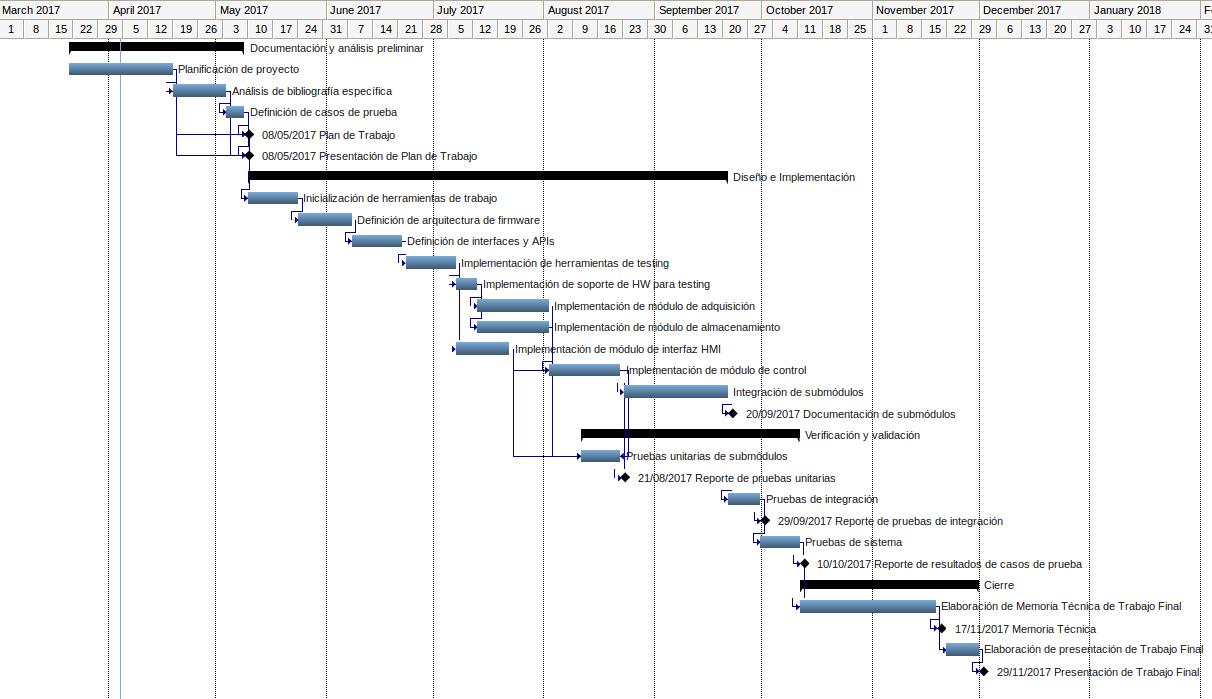
\includegraphics[height=.85\textheight]{./Figuras/Gantt-2.png}
\caption{Ejemplo de diagrama de Gantt (apaisado).} %Modificar este título acorde.
\label{fig:diagGantt}
\end{figure}

\end{landscape}

\end{consigna}


\section{12. Presupuesto detallado del proyecto}
\label{sec:presupuesto}

\begin{consigna}{red}
Si el proyecto es complejo entonces separarlo en partes:
\begin{itemize}
	\item Un total global, indicando el subtotal acumulado por cada una de las áreas.
	\item El desglose detallado del subtotal de cada una de las áreas.
\end{itemize}

IMPORTANTE: No olvidarse de considerar los COSTOS INDIRECTOS.

Incluir la aclaración de si se emplea como moneda el peso argentino (ARS) o si se usa moneda extranjera (USD, EUR, etc). Si es en moneda extranjera se debe indicar la tasa de conversión respecto a la moneda local en una fecha dada.

\end{consigna}

\begin{table}[htpb]
\centering
\begin{tabularx}{\linewidth}{@{}|X|c|r|r|@{}}
\hline
\rowcolor[HTML]{C0C0C0} 
\multicolumn{4}{|c|}{\cellcolor[HTML]{C0C0C0}COSTOS DIRECTOS} \\ \hline
\rowcolor[HTML]{C0C0C0} 
Descripción &
  \multicolumn{1}{c|}{\cellcolor[HTML]{C0C0C0}Cantidad} &
  \multicolumn{1}{c|}{\cellcolor[HTML]{C0C0C0}Valor unitario} &
  \multicolumn{1}{c|}{\cellcolor[HTML]{C0C0C0}Valor total} \\ \hline
 &
  \multicolumn{1}{c|}{} &
  \multicolumn{1}{c|}{} &
  \multicolumn{1}{c|}{} \\ \hline
 &
  \multicolumn{1}{c|}{} &
  \multicolumn{1}{c|}{} &
  \multicolumn{1}{c|}{} \\ \hline
\multicolumn{1}{|l|}{} &
   &
   &
   \\ \hline
\multicolumn{1}{|l|}{} &
   &
   &
   \\ \hline
\multicolumn{3}{|c|}{SUBTOTAL} &
  \multicolumn{1}{c|}{} \\ \hline
\rowcolor[HTML]{C0C0C0} 
\multicolumn{4}{|c|}{\cellcolor[HTML]{C0C0C0}COSTOS INDIRECTOS} \\ \hline
\rowcolor[HTML]{C0C0C0} 
Descripción &
  \multicolumn{1}{c|}{\cellcolor[HTML]{C0C0C0}Cantidad} &
  \multicolumn{1}{c|}{\cellcolor[HTML]{C0C0C0}Valor unitario} &
  \multicolumn{1}{c|}{\cellcolor[HTML]{C0C0C0}Valor total} \\ \hline
\multicolumn{1}{|l|}{} &
   &
   &
   \\ \hline
\multicolumn{1}{|l|}{} &
   &
   &
   \\ \hline
\multicolumn{1}{|l|}{} &
   &
   &
   \\ \hline
\multicolumn{3}{|c|}{SUBTOTAL} &
  \multicolumn{1}{c|}{} \\ \hline
\rowcolor[HTML]{C0C0C0}
\multicolumn{3}{|c|}{TOTAL} &
   \\ \hline
\end{tabularx}%
\end{table}


\section{13. Gestión de riesgos}
\label{sec:riesgos}

\begin{consigna}{red}
a) Identificación de los riesgos (al menos cinco) y estimación de sus consecuencias:
 
Riesgo 1: detallar el riesgo (riesgo es algo que si ocurre altera los planes previstos de forma negativa)
\begin{itemize}
	\item Severidad (S): mientras más severo, más alto es el número (usar números del 1 al 10).\\
	Justificar el motivo por el cual se asigna determinado número de severidad (S).
	\item Probabilidad de ocurrencia (O): mientras más probable, más alto es el número (usar del 1 al 10).\\
	Justificar el motivo por el cual se asigna determinado número de (O). 
\end{itemize}   

Riesgo 2:
\begin{itemize}
	\item Severidad (S): X.\\
	Justificación...
	\item Ocurrencia (O): Y.\\
	Justificación...
\end{itemize}

Riesgo 3:
\begin{itemize}
	\item Severidad (S):  X.\\
	Justificación...
	\item Ocurrencia (O): Y.\\
	Justificación...
\end{itemize}


b) Tabla de gestión de riesgos:      (El RPN se calcula como RPN=SxO)

\begin{table}[htpb]
\centering
\begin{tabularx}{\linewidth}{@{}|X|c|c|c|c|c|c|@{}}
\hline
\rowcolor[HTML]{C0C0C0} 
Riesgo & S & O & RPN & S* & O* & RPN* \\ \hline
       &   &   &     &    &    &      \\ \hline
       &   &   &     &    &    &      \\ \hline
       &   &   &     &    &    &      \\ \hline
       &   &   &     &    &    &      \\ \hline
       &   &   &     &    &    &      \\ \hline
\end{tabularx}%
\end{table}

Criterio adoptado: 

Se tomarán medidas de mitigación en los riesgos cuyos números de RPN sean mayores a...

Nota: los valores marcados con (*) en la tabla corresponden luego de haber aplicado la mitigación.

c) Plan de mitigación de los riesgos que originalmente excedían el RPN máximo establecido:
 
Riesgo 1: plan de mitigación (si por el RPN fuera necesario elaborar un plan de mitigación).
  Nueva asignación de S y O, con su respectiva justificación:
  \begin{itemize}
	\item Severidad (S*): mientras más severo, más alto es el número (usar números del 1 al 10).
          Justificar el motivo por el cual se asigna determinado número de severidad (S).
	\item Probabilidad de ocurrencia (O*): mientras más probable, más alto es el número (usar del 1 al 10).
          Justificar el motivo por el cual se asigna determinado número de (O).
	\end{itemize}

Riesgo 2: plan de mitigación (si por el RPN fuera necesario elaborar un plan de mitigación).
 
Riesgo 3: plan de mitigación (si por el RPN fuera necesario elaborar un plan de mitigación).

\end{consigna}


\section{14. Gestión de la calidad}
\label{sec:calidad}

\begin{consigna}{red}
Elija al menos diez requerimientos que a su criterio sean los más importantes/críticos/que aportan más valor y para cada uno de ellos indique las acciones de verificación y validación que permitan asegurar su cumplimiento.

\begin{itemize} 
\item Req \#1: copiar acá el requerimiento con su correspondiente número.

\begin{itemize}
	\item Verificación para confirmar si se cumplió con lo requerido antes de mostrar el sistema al cliente. Detallar.
	\item Validación con el cliente para confirmar que está de acuerdo en que se cumplió con lo requerido. Detallar. 
\end{itemize}

\end{itemize}

Tener en cuenta que en este contexto se pueden mencionar simulaciones, cálculos, revisión de hojas de datos, consulta con expertos, mediciones, etc.  

Las acciones de verificación suelen considerar al entregable como ``caja blanca'', es decir se conoce en profundidad su funcionamiento interno.  

En cambio, las acciones de validación suelen considerar al entregable como ``caja negra'', es decir, que no se conocen los detalles de su funcionamiento interno.

\end{consigna}

\section{15. Procesos de cierre}    
\label{sec:cierre}

\begin{consigna}{red}
Establecer las pautas de trabajo para realizar una reunión final de evaluación del proyecto, tal que contemple las siguientes actividades:

\begin{itemize}
	\item Pautas de trabajo que se seguirán para analizar si se respetó el Plan de Proyecto original:\\
	 - Indicar quién se ocupará de hacer esto y cuál será el procedimiento a aplicar. 
	\item Identificación de las técnicas y procedimientos útiles e inútiles que se emplearon, los problemas que surgieron y cómo se solucionaron:\\
	 - Indicar quién se ocupará de hacer esto y cuál será el procedimiento para dejar registro.
	\item Indicar quién organizará el acto de agradecimiento a todos los interesados, y en especial al equipo de trabajo y colaboradores:\\
	  - Indicar esto y quién financiará los gastos correspondientes.
\end{itemize}

\end{consigna}

\end{document}